\documentclass[11pt]{article}
\usepackage[margin=1in]{geometry}
\usepackage{graphicx}
\usepackage{booktabs}
\usepackage{amsmath}
\usepackage{amssymb}
\usepackage[hidelinks]{hyperref}
\graphicspath{{figures/}}

\title{Supplementary Information\\[0.3em]
\large Architecture-dependent effects of imbalance correction in melanoma classification: a controlled audit with fairness, calibration, and explanation analysis}
\author{}
\date{}

\begin{document}
\maketitle

\section*{S1 Per-seed Stage 2 metrics}

Table~\ref{tab:suppstage2} reports every Stage 2 run. The main text reports seed-level means and 95\% t intervals.

\begin{table}[h]
\centering
\small
\caption{Per-seed Stage 2 test metrics at the validation-selected 95\% specificity threshold.}
\label{tab:suppstage2}
\begin{tabular}{llcccc}
\toprule
Architecture & Condition & Seed & Sensitivity & Specificity & AUC \\
\midrule
ResNet-50 & CE & 1 & 0.608 & 0.944 & 0.896 \\
ResNet-50 & CE & 2 & 0.527 & 0.961 & 0.901 \\
ResNet-50 & CE & 3 & 0.575 & 0.949 & 0.895 \\
ResNet-50 & CE+strong & 1 & 0.602 & 0.936 & 0.910 \\
ResNet-50 & CE+strong & 2 & 0.554 & 0.943 & 0.890 \\
ResNet-50 & CE+strong & 3 & 0.548 & 0.948 & 0.897 \\
ResNet-50 & Focal+CB & 1 & 0.435 & 0.943 & 0.881 \\
ResNet-50 & Focal+CB & 2 & 0.398 & 0.955 & 0.885 \\
ResNet-50 & Focal+CB & 3 & 0.527 & 0.942 & 0.887 \\
EfficientNet-B0 & CE & 1 & 0.543 & 0.956 & 0.917 \\
EfficientNet-B0 & CE & 2 & 0.527 & 0.949 & 0.905 \\
EfficientNet-B0 & CE & 3 & 0.597 & 0.955 & 0.920 \\
EfficientNet-B0 & CE+strong & 1 & 0.570 & 0.952 & 0.909 \\
EfficientNet-B0 & CE+strong & 2 & 0.624 & 0.946 & 0.922 \\
EfficientNet-B0 & CE+strong & 3 & 0.495 & 0.957 & 0.905 \\
EfficientNet-B0 & Focal+CB & 1 & 0.522 & 0.947 & 0.884 \\
EfficientNet-B0 & Focal+CB & 2 & 0.392 & 0.946 & 0.882 \\
EfficientNet-B0 & Focal+CB & 3 & 0.516 & 0.955 & 0.907 \\
ViT-S/16 & CE & 1 & 0.349 & 0.949 & 0.850 \\
ViT-S/16 & CE & 2 & 0.430 & 0.937 & 0.842 \\
ViT-S/16 & CE & 3 & 0.419 & 0.938 & 0.870 \\
ViT-S/16 & CE+strong & 1 & 0.349 & 0.942 & 0.853 \\
ViT-S/16 & CE+strong & 2 & 0.516 & 0.942 & 0.877 \\
ViT-S/16 & CE+strong & 3 & 0.441 & 0.938 & 0.868 \\
ViT-S/16 & Focal+CB & 1 & 0.505 & 0.944 & 0.878 \\
ViT-S/16 & Focal+CB & 2 & 0.462 & 0.928 & 0.860 \\
ViT-S/16 & Focal+CB & 3 & 0.478 & 0.948 & 0.880 \\
\bottomrule
\end{tabular}
\end{table}


\section*{S2 XAI error-type mass}

Table~\ref{tab:suppxai} reports attribution mass for false negatives and false positives with Grad-CAM targeting the true class. The values do not separate consistently across architectures.

\begin{table}[h]
\centering
\small
\caption{Attribution mass by error type for the true-class Grad-CAM analysis. Values are means across images and seeds.}
\label{tab:suppxai}
\begin{tabular}{llcc}
\toprule
Architecture & Error type & Images & Attribution mass \\
\midrule
EfficientNet-B0 & FN & 23 & 0.374 \\
EfficientNet-B0 & FP & 31 & 0.260 \\
ResNet-50 & FN & 22 & 0.346 \\
ResNet-50 & FP & 25 & 0.349 \\
ViT-S/16 & FN & 30 & 0.420 \\
ViT-S/16 & FP & 31 & 0.344 \\
\bottomrule
\end{tabular}
\end{table}


\section*{S3 Training and ROC figures}

Figures~\ref{fig:supptraining} and~\ref{fig:supproc} show the training curves and test ROC curve for the median seed of ResNet-50 with the CE baseline. These figures were moved out of the main text because they are illustrative and were generated at 150 dpi.

\begin{figure}[h]
  \centering
  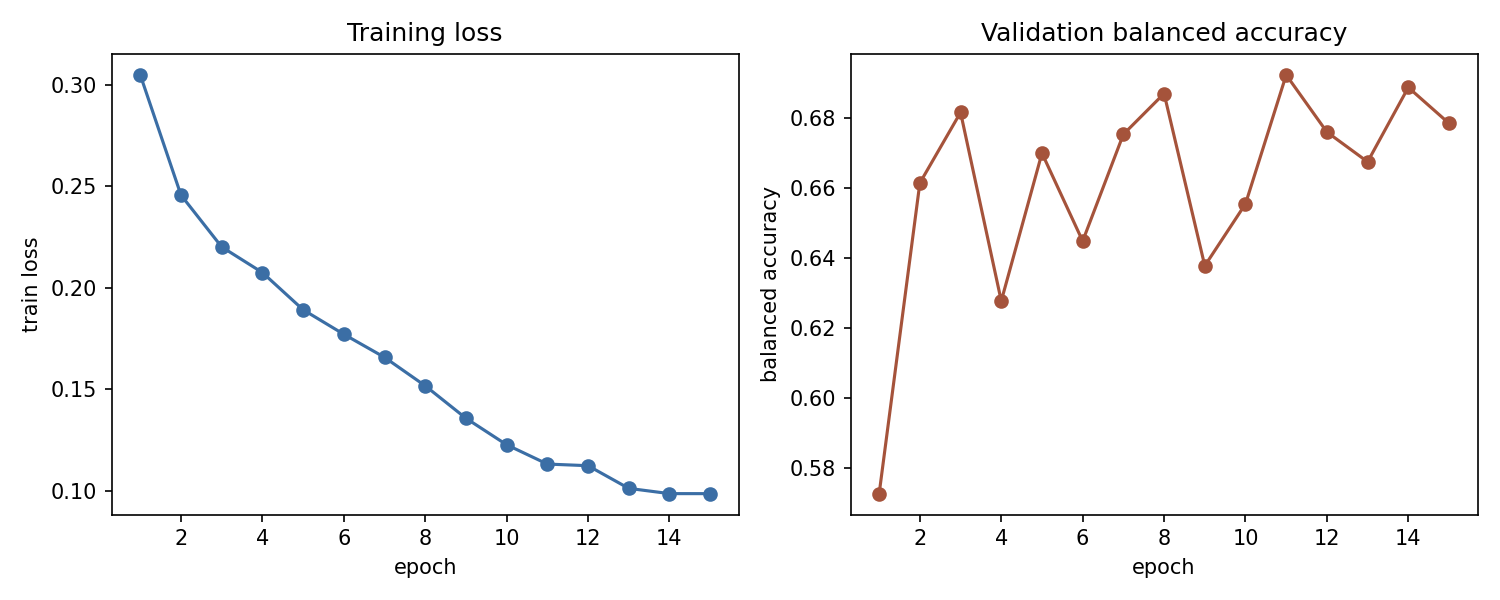
\includegraphics[width=\linewidth]{stage2_best_sensitivity_training_curves.png}
  \caption{Training loss and validation balanced accuracy for the median seed of ResNet-50 with the CE baseline.}
  \label{fig:supptraining}
\end{figure}

\begin{figure}[h]
  \centering
  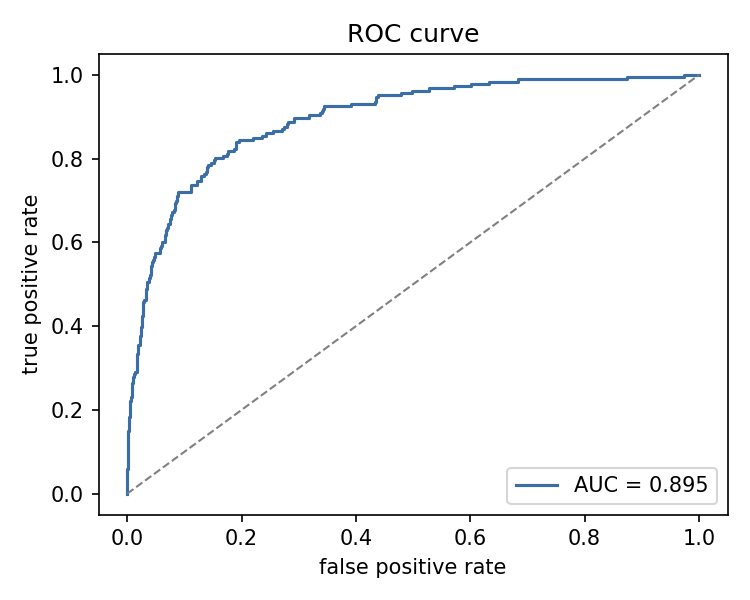
\includegraphics[width=0.72\linewidth]{stage2_best_sensitivity_roc_test.png}
  \caption{Test ROC curve for the median seed of ResNet-50 with the CE baseline. The operating threshold is selected on validation at 95\% specificity.}
  \label{fig:supproc}
\end{figure}

\section*{S4 Data, code, and additional results}

The lesion-aware split is released as \texttt{results/split\_ham10000\_lesion\_seed42.csv}. Per-sample test predictions for all 27 runs are in \texttt{results/predictions/}. The full adjusted-model coefficients, dark-skin AUC comparisons, calibration summaries, and XAI metrics are available from the corresponding author upon reasonable request. The repository link is withheld for double-blind review.

\end{document}
